\documentclass[]{article}
\usepackage{lmodern}
\usepackage{amssymb,amsmath}
\usepackage{ifxetex,ifluatex}
\usepackage{fixltx2e} % provides \textsubscript
\ifnum 0\ifxetex 1\fi\ifluatex 1\fi=0 % if pdftex
  \usepackage[T1]{fontenc}
  \usepackage[utf8]{inputenc}
\else % if luatex or xelatex
  \ifxetex
    \usepackage{mathspec}
    \usepackage{xltxtra,xunicode}
  \else
    \usepackage{fontspec}
  \fi
  \defaultfontfeatures{Mapping=tex-text,Scale=MatchLowercase}
  \setromanfont{TeX Gyre Pagella}
  \newcommand{\euro}{€}
\fi
% use upquote if available, for straight quotes in verbatim environments
\IfFileExists{upquote.sty}{\usepackage{upquote}}{}
% use microtype if available
\IfFileExists{microtype.sty}{%
\usepackage{microtype}
\UseMicrotypeSet[protrusion]{basicmath} % disable protrusion for tt fonts
}{}
\usepackage[margin=1in]{geometry}
\usepackage{longtable,booktabs}
\usepackage{graphicx}
\makeatletter
\def\maxwidth{\ifdim\Gin@nat@width>\linewidth\linewidth\else\Gin@nat@width\fi}
\def\maxheight{\ifdim\Gin@nat@height>\textheight\textheight\else\Gin@nat@height\fi}
\makeatother
% Scale images if necessary, so that they will not overflow the page
% margins by default, and it is still possible to overwrite the defaults
% using explicit options in \includegraphics[width, height, ...]{}
\setkeys{Gin}{width=\maxwidth,height=\maxheight,keepaspectratio}
\ifxetex
  \usepackage[setpagesize=false, % page size defined by xetex
              unicode=false, % unicode breaks when used with xetex
              xetex]{hyperref}
\else
  \usepackage[unicode=true]{hyperref}
\fi
\hypersetup{breaklinks=true,
            bookmarks=true,
            pdfauthor={M. Callaghan and V. Niberg},
            pdftitle={Twitter and the European Hyperagora: What can the Twittersphere Tell us about Political Deliberation and Opinions in Europe?},
            colorlinks=true,
            citecolor=blue,
            urlcolor=blue,
            linkcolor=magenta,
            pdfborder={0 0 0}}
\urlstyle{same}  % don't use monospace font for urls
\usepackage{url}

\setlength{\parindent}{0pt}
\setlength{\parskip}{6pt plus 2pt minus 1pt}
\setlength{\emergencystretch}{3em}  % prevent overfull lines
\setcounter{secnumdepth}{0}

%%% Use protect on footnotes to avoid problems with footnotes in titles
\let\rmarkdownfootnote\footnote%
\def\footnote{\protect\rmarkdownfootnote}

%%% Change title format to be more compact
\usepackage{titling}

% Create subtitle command for use in maketitle
\newcommand{\subtitle}[1]{
  \posttitle{
    \begin{center}\large#1\end{center}
    }
}

\setlength{\droptitle}{-2em}
  \title{Twitter and the European Hyperagora: What can the Twittersphere Tell us
about Political Deliberation and Opinions in Europe?}
  \pretitle{\vspace{\droptitle}\centering\huge}
  \posttitle{\par}
  \author{M. Callaghan and V. Niberg}
  \preauthor{\centering\large\emph}
  \postauthor{\par}
  \predate{\centering\large\emph}
  \postdate{\par}
  \date{December 11, 2015}



\begin{document}

\maketitle


{
\hypersetup{linkcolor=black}
\setcounter{tocdepth}{2}
\tableofcontents
}
\newpage

\section{Introduction}\label{introduction}

Twitter is an online social network that allows users to broadcast short
posts known as Tweets. Since its launch in 2006, the platform has
increasingly been used for everyday communication as well as for
political debates, crisis communication, marketing, and cultural
participation (Weller et al. 2013). The public-debt crisis in Europe is
widely discussed across Europe and presents an interesting point in time
to investigate whether European issues are discussed in a common
European public sphere. This project looks at data from the
communication platform Twitter. It specifically looks at the reaction in
the Twittersphere to the negotiation between the Troika and Greece
leading up to the signing of the three memorandums.

\section{Research Question}\label{research-question}

The following questions were investigated:

What can twitter tell us about pan-European reactions to the European
governance of the public-debt crisis in Greece?

\begin{itemize}
\item
  What can variation across time and space in the volume of Tweets
  regarding the euro crisis tell us about popular engagement with the
  issues?
\item
  What can the content of Tweets related to the crisis tell us about the
  spread of public opinion on the handling of the crisis in Greece
  between and within countries?
\end{itemize}

The answer to these questions could potentially add to the literature on
the emergence of a European public sphere.

\section{Literature Review}\label{literature-review}

\subsection{On Twitter Research}\label{on-twitter-research}

The body of twitter research has grown steadily in recent years (for a
comprehensive analysis and typology of twitter research up to 2013, see
Zimmer and Proferes 2014). Some of the findings relevant to our research
design are discussed below.

Twitter is a source of meaningful information about engagement with and
opinions about political topics. Twitter is also used as a platform for
political deliberation. In a recent study on Tweets mentioning parties
or politicians before the 2009 German federal election, Tumasjan et al.
found that ``Twitter is not just used to spread political opinions, but
also to discuss these opinions with other users'' (Tumasjan et al. 2010,
183). Furthermore, specific patterns of twitter usage have been
identifed that correspond with high-profile political events. Hughes and
Palen found that, compared to general Twitter usage, more
broadcast-based information sharing activities take place (Hughes and
Palen 2009, 259) during events. Moreover, Tumasjan et al. found that it
was possible to extact meaningful information about political opinions
from both the volumes and the content of these Tweets: ``the mere number
of Tweets reflects voter preferences and came close to traditional
election polls'' (Tumasjan et al. 2010, 183).

Twitter gives information on the location of Tweets and users, which
must be carefully interpreted. Devin Gaffney points out methodological
problems with using the given location of twitter users - ``in many
cases user-entered profile locations differ from the physical locations
users are actually Tweeting from'' (Graham, Hale, and Gaffney,Devin
2014, 1) which must be considered when interepreteing results.

Though the field of Sentiment Analysis (SA) is perhaps most developed in
the business world (Zimmer and Proferes 2014, 250), an increasing body
of literature has developed, focused on retrieving information about
political opinions from the Twittersphere. Though Tumasjan's results
have come under scrutiny (see Jungherr, J{ü}rgens, and Schoen 2012), the
authors found that ``the sentiment of Twiter messages closely
corresponded to political programs, candidate profiles, and evidence
from the media coverage of the campaign trail'' (Tumasjan et al. 2010,
183).

Grimmer provides an overview of recent developments in SA in political
science, noting how ``automated content methods can make possible the
previously impossible in political science: the systematic analysis of
large-scale text collections without massive funding support'' (Grimmer
and Stewart 2013, 2). He advises caution, however, about the utility of
SA in predictive models: ``The goal of building text models is therefore
different than model building to make causal inferences. {[}\ldots{}{]}
Emphasis in evaluations should be placed on helping researchers to
assign documents into predetermined categories, discover new and useful
categorizytion schemes for texts, or in measuring theoretically relevant
quantities from large collections of text.'' (Grimmer and Stewart 2013,
4).

Due to the enourmous amount of text available, Pak and Paroubek identify
that ``microblogging web-sites are rich sources of data for opinion
mining and sentiment analysis'' (Pak and Paroubek 2010, 1320). The
multilingual nature of Tweets across Europe presents some difficulties,
but is the subject of a growing body of research: ``Noisy social media,
such as Twitter, are especially interesting for sentiment analysis (SA)
{[}\ldots{}{]} given the amount of data and their popularity in
different countries, where users simultaneously publish opinions about
the same topic in different languages'' (Vilares, Alonso, and
G{ó}mez-Rodr{i}guez 2015, 2). Balahur and Turchi are confident about the
ability of Statistical Machine Translation (SMT) to provide a basis for
consistently applied SA across languages (Balahur and Turchi 2012, 58).
Other approaches include using emoticons to train models that assign
sentiment to a multilingual text corpus (Narr, Hulfenhaus, and Albayrak
2012).

Finally, some studies discuss ethical aspects of twitter research. For
example, concerns about creating a permanent archive of Tweets have been
voiced. These concerns included whether ``such archive was aligned with
users' privacy expectations'' (Zimmer and Proferes 2014, 258; Zimmer
2010).

\subsection{On Awareness and Public Opinion across Europe on the
Governance of the Public-Debt Crisis in
Greece}\label{on-awareness-and-public-opinion-across-europe-on-the-governance-of-the-public-debt-crisis-in-greece}

Academic research on the emergence of a European public sphere is not a
recent phenomenon (Risse 2003, 1). Hitherto, however, research has been
characterized as rather normative, as the ``research community has been
{[}\ldots{}{]} interested in producing policy recommendations for public
sphere-building'' (Trenz 2015, 234). Recent studies, on the other hand,
seem to put emphasis on an empirical grounding of the debate (Trenz
2015; Drewski, Gerhards, and others 2015). This development is being
mirrored in research on the public debate across Europe on the euro
crisis. It has been suggested that ``there is an emerging demos in the
European polity and it has been strengthened during the euro crisis''
(Risse 2014, 1213). When testing this hypothesis empirically, though, by
looking at newspaper editorials in Spain and Germany, Drewski found that
there were significant differences along national instead of ideological
lines in the discussion of the Euro crisis (Drewski, Gerhards, and
others 2015, 5).

Max Hänska and Stefan Bauchowitz in a recent LSE blog entry track
twitter activity during the negotiations leading up to the third Greek
bailout agreement. (Haenska and Bauchowitz 2015) According to their
findings, Tweets synchronised around key mini-events throughout the
negotiations, with peaks and troughs mirrored across national
twitter-spheres. These results suggest that popular engagement with the
issue converges across Europe (see figure 1).

\begin{figure}[htbp]
\centering
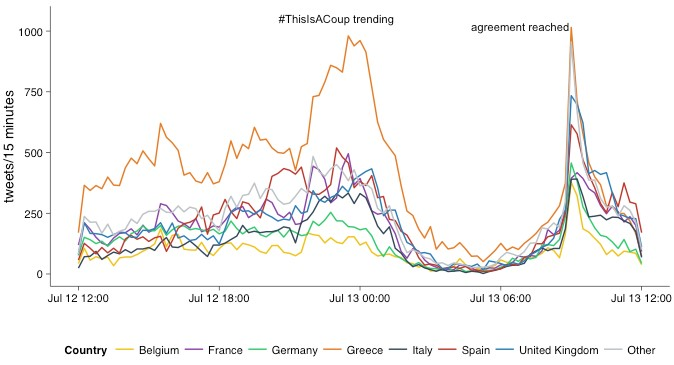
\includegraphics{../../img/Greece-twitter-1.jpg}
\caption{Tweet volumes by country on 12-13 July 2015 in European
countries (source Haenska and Bauchowitz 2015)}
\end{figure}

They further looked at instances of Tweets containing \#ThisIsACoup,
representing a particular opinion on the agreement. They then showed
that the spread of \#ThisIsACoup was not reflected in the studied
countries equally. This indicated a divergence of public opinion along
national lines (see figure 2).

\begin{figure}[htbp]
\centering
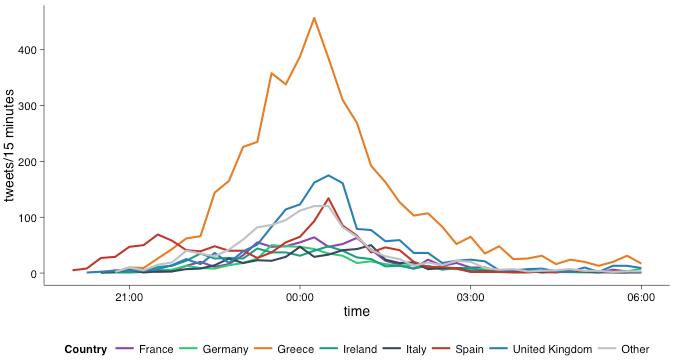
\includegraphics{../../img/Greece-twitter-2.png}
\caption{Number of Tweets containing the \#thisisacoup hashtag on 12-13
July 2015 (source Haenska and Bauchowitz 2015)}
\end{figure}

However, figure 3 shows how tweets across Europe were connected.

\begin{figure}[htbp]
\centering
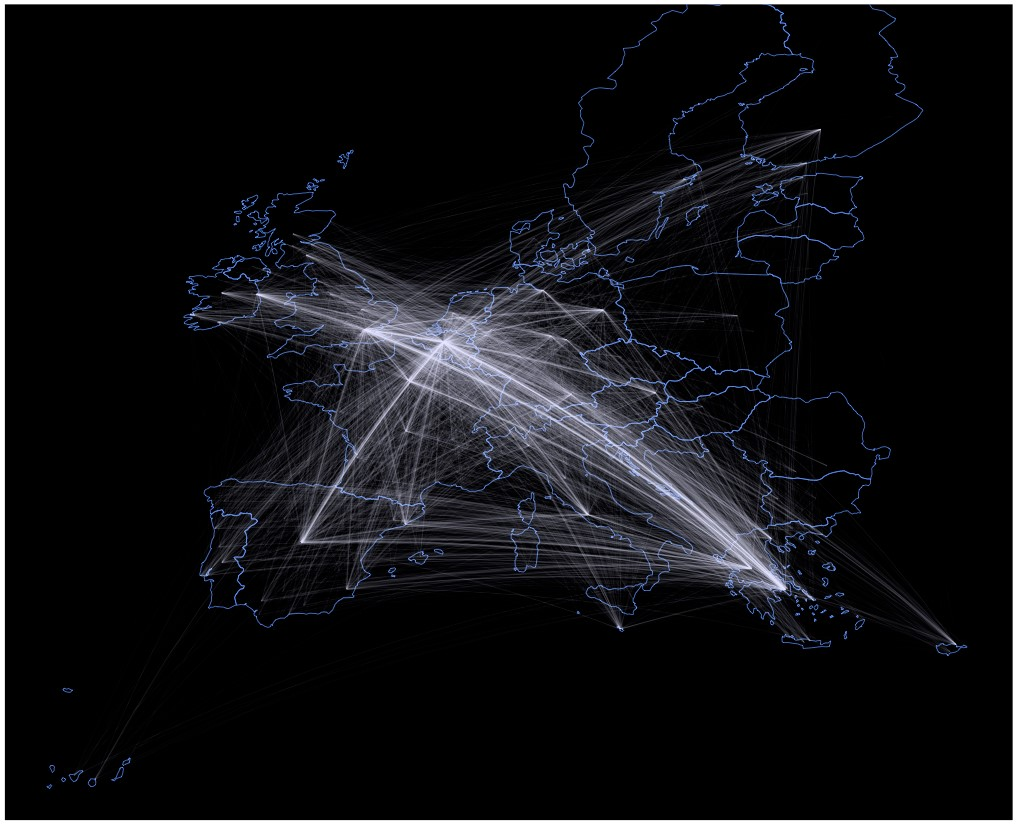
\includegraphics{../../img/Greece-twitter-3.jpg}
\caption{A network map of European tweets (source Haenska and Bauchowitz
2015)}
\end{figure}

\section{Data Sources}\label{data-sources}

For our investigation in the European public discourse on the Euro
crisis, two datasets were required. The first was the corpus of Tweets
relating to the Greek debt crisis and the measures taken to manage the
crisis by European institutions. The second was information about the
users whose Tweets form the body of that corpus.

Zimmer and Proferes identify the Library of Congress' decision to place
every Tweet since Twitter's inception in 2006 into an archive as
validating ``the research importance of twitter'' (Zimmer and Proferes
2014, 251). Despite this announcement occuring in 2010, five years
later, the archive is still not open to researchers (Scola 2015). Since
late 2014, the whole corpus of twitter data has been searchable online
(Metz 2015). Programmatic access to this archive is, however, more
restricted. Twitter's public search API ``is not complete index of all
Tweets, but instead an index of recent Tweets. At the moment that index
includes between 6-9 days of Tweets.'' (``The Search API'' 2015).
Twitter sells access to historical Tweets through an API provided by its
``enterprise API platform'' GNIP (Tornes 2015). This paper adapts a
publicly available program written in Java which scrapes results from
Twitter's online search page (Henrique 2015).

\subsection{Data Gathering}\label{data-gathering}

Due to the large amount of data we process, we ran the data gathering
and cleaning in the background on a server using the prefix setsid.

\subsubsection{Tweets}\label{tweets}

We used a modified version of GetOldTweets (Henrique 2015), a Java
program that scrapes data from twitter search. The file
getting\_tweets/input.txt contains a list of search terms related to the
Greek crisis in three periods, each comprising some weeks before and
after the negotiation and signing of the memoranda. The search terms
were collected using an adapted form of snowball sampling (Biernacki and
Waldorf 1981), searching an initial list and recursively adding related
terms found in the results. By running

\begin{verbatim}
sudo setsid ./compile_run.sh ../getting_tweets/input.txt
\end{verbatim}

from the GetOldTweets folder, we ran through each search term and each
period, searched twitter, and saved the results as a txt file in the
data folder. After an initial assessment of the results, we refined our
search terms and ran GetOldTweets again with
/getting\_tweets/input2.txt. A third file (getting\_tweets/input3.txt)
aims to return a time-inpedependent list of tweets in order to control
for the growth of Twitter over time.

We end up with a long list of files in the data/GOToutput folder, which
in the data cleaning process will be merged into one corpus file.

\subsubsection{Users}\label{users}

We found the unique users in our corpus of tweets and used the TwitteR
package (Gentry 2015) to gather richer data about each user. TwitteR
uses the twitter API and gives the opportunity to collect all
information twitter has abou the user. Where a users's last tweet was
geocoded, we took the latitude and longtitude. We end up with the file
data/user\_info.csv

Many users do not geotag their tweets, instead stating their location,
and we used APIs from MapQuest and Google to geocode user-reported
location, giving us the file places.csv.

\subsection{Merging \& Cleaning}\label{merging-cleaning}

The txt files containing the tweets for each query and period are merged
into a corpus file. This corpus file was merged with the user\_info
file, which in turn was merged with the places file. We end up with a
large file containing tweets for our queries in each period with
elaborete user information.

Some of the queries we defined returned irrelevant data, due to their
ambiguity. We identified these by selecting random tweets from the
search queries, reading the tweets, and checking for relevance to the
topic. For example, the query ``bailout'', although certainly relevant
for our topic, was insufficiently precise and returned a lot of data
about the banking bailouts, especially in the 2010 period. The following
list summarizes the queries which we excluded.

\begin{itemize}
\itemsep1pt\parskip0pt\parsep0pt
\item
  athens
\item
  bailout
\item
  2-pac
\item
  3-pac
\end{itemize}

\subsection{Translation}\label{translation}

In a next step we identified the language of every tweet (Hornik et al.
2015) and translated those tweets written in European languages other
than English into English (Lucas and Tingley 2014). Danish and Romanian
were excluded from the list because these languages were not adequately
identified by the program.

\subsection{Final Dataset}\label{final-dataset}

A dataframe `merged\_corpus' containing all of the above information was
pulled together. We filtered all tweets from Europe.

\section{Methodology}\label{methodology}

Volumes of topic-relevant Tweets were mapped across space and time, to
analyse the distribution of topic-awareness and its relation to
political developments in responses to the crisis. The distribution of
hashtags that clearly represent an opinion on the response to the crisis
(e.g. `\#ThisIsaCoup', `\#ThisIsNotaCoup' \emph{inter alia}) were
similarly mapped in order to approximate the distribution of opinion
within and between countries over time. The paper attempts a sentiment
analysis of Tweets expressing opinions about the agreed bailout deals
using machine translation to translate all texts into English before
performing sentiment analysis. Analysis was then carried out using
unigrams to indicate polarity through comparison with a lexicon.
Following Grimmer, we assumed ``documents are a \emph{bag of words},
where order does not inform our analyses'' as ``In practice, for common
tasks like measuring sentiment, topic modeling, or search,
\emph{n-grams} (combinations of words rather than individual words) do
little to enhance performance'' (Grimmer and Stewart 2013, 6).

To carry out the sentiment analysis process, we use the R package
tm.plugin.sentiment (Annau 2014) to compare the words in our translated
corpus of tweets with the General Enquirer lecixon (Theussl, Hofmarcher,
and Hornik 2015). Each tweets is given a positive score and a negative
score according to the number of positive and negative words found in
the tweet. We calculate an overall sentiment score by subtracting the
negative score from the positive score. Low scores therefore indicate
negative sentiment; high scores indicate positive sentiment.

Based on the results of sentiment analysis carried out and analysis of
volumes of tweets and users using opinion-signifying keywords, the paper
gives an indication of the scale of dialogue, consensus and disagreement
across and within countries in the European Twittersphere.

\section{Analysis}\label{analysis}

\subsection{Descriptive Statistics}\label{descriptive-statistics}

The word cloud gives us an overall picture of the words used in the
collected tweets connected to the European public-debt crisis.\footnote{to
  a certain degree in this case a word cloud is redundant, because it
  mainly returns our query turns. However, it also indicates the
  prevalence of specific terms, and further, which other terms are
  mentioned regularly in those tweets.}

\begin{figure}[htbp]
\centering
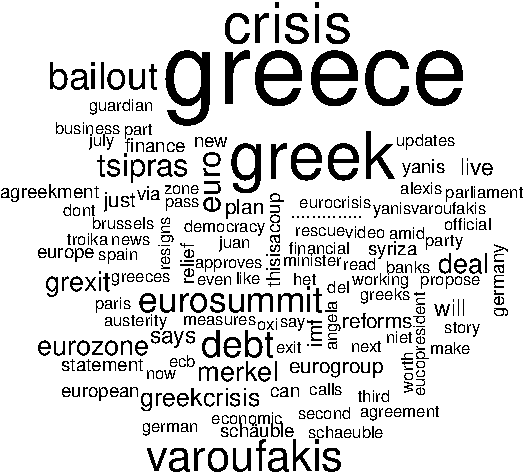
\includegraphics{fin_paper_files/figure-latex/unnamed-chunk-2-1.pdf}
\caption{Word Cloud of a random sample of 200 tweets in our corpus}
\end{figure}

The following tables describe variation over space and time of the
entire population of tweets.

\subsubsection{Variation Across Space}\label{variation-across-space}

\begin{figure}

{\centering 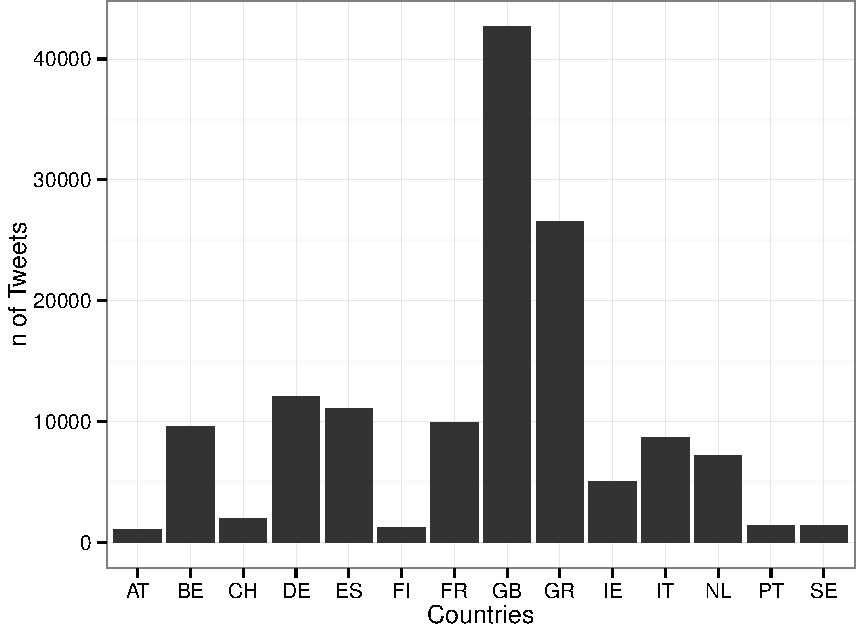
\includegraphics{fin_paper_files/figure-latex/unnamed-chunk-3-1} 

}

\caption{Geographical Distribution of Tweets}\label{fig:unnamed-chunk-3}
\end{figure}

Figure 5 shows the distribution of all tweets over countries filtering
those with a significant amount of tweets. This group seems to be a mix
of high twitter user numbers and affectedness/involvement/relation to
the events in Greece. Most probably reflecting high user numbers in the
US, the US seems to be the origin of most tweets regarding the European
sovereign-debt crisis. However, when controlling for period, the US
resembles an atypical case. While for most other countries, tweet number
on the topic increase over the years, they decrease substantially in the
US.

\subsubsection{Variation Across Time}\label{variation-across-time}

\begin{figure}

{\centering 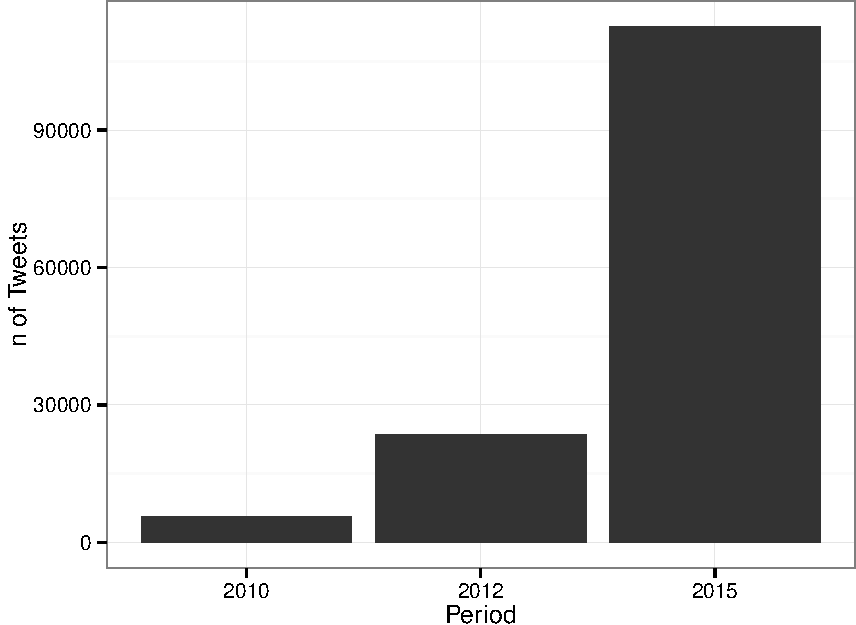
\includegraphics{fin_paper_files/figure-latex/unnamed-chunk-4-1} 

}

\caption{Tweets matching our queries by year}\label{fig:unnamed-chunk-4}
\end{figure}

Figure 6 shows that twitter coverage of the Greek bailouts has increased
heavily over time. When looking at the development of different queries
over time, an increase was found for all queries except for for
``imf+greece'', which decreased in 2012 and increased in 2015 again.
Since the shown results are not normalized, it is difficult to say how
much of the growth of the population of tweets can be attributed to an
increase in twitter usage or to an increase of interest in the topic.
Further, some of our queries only became topical in the later periods or
even the last periods.

\subsubsection{Variation Across Space and
Time}\label{variation-across-space-and-time}

Figure 7 Shows us that tweets in earlier periods are concentrated in
very few countries. Only in 2015 do we see a wider distribution across
all European countries.

\begin{figure}

{\centering 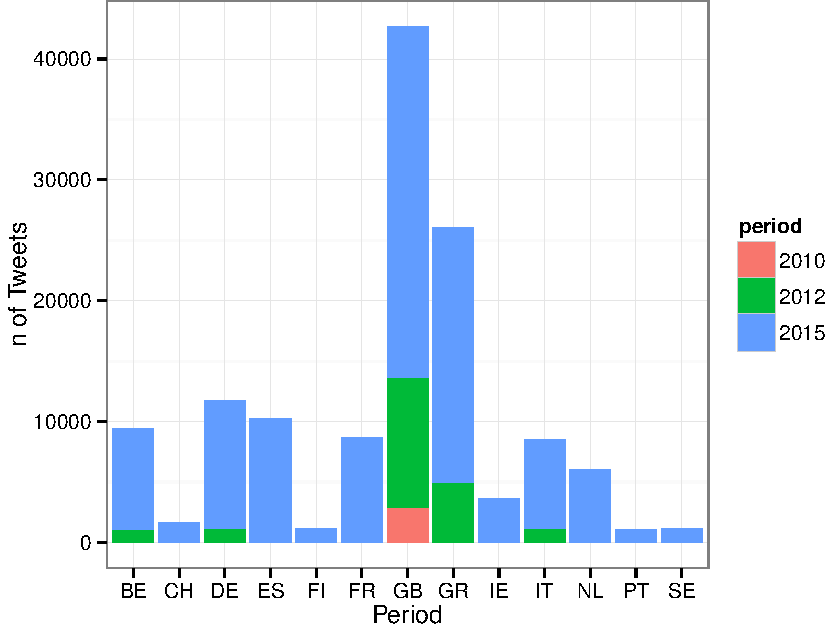
\includegraphics{fin_paper_files/figure-latex/unnamed-chunk-5-1} 

}

\caption{Spatio-Temporal distribution of total tweets in corpus}\label{fig:unnamed-chunk-5}
\end{figure}

\subsection{Queries}\label{queries}

Table 1 summarizes the collected data by queries. It shows absolute
numbers and relative distributions of specific query returns.

\begin{longtable}[c]{@{}lrr@{}}
\caption{Data distribution by query}\tabularnewline
\toprule
query & n & percent\tabularnewline
\midrule
\endfirsthead
\toprule
query & n & percent\tabularnewline
\midrule
\endhead
\#aGreekment & 3045 & 2.15\tabularnewline
athens+berlin & 478 & 0.34\tabularnewline
austerity+greece & 2833 & 2.00\tabularnewline
economic+adjustment & 55 & 0.04\tabularnewline
eucrisis & 117 & 0.08\tabularnewline
eurocrisis & 2582 & 1.82\tabularnewline
eurogroup & 1421 & 1.00\tabularnewline
eurogroup+agreement & 312 & 0.22\tabularnewline
eurosummit & 8969 & 6.33\tabularnewline
euro+summit & 10211 & 7.20\tabularnewline
germany+greece & 3861 & 2.72\tabularnewline
greece+crisis & 3591 & 2.53\tabularnewline
greece+reforms & 4297 & 3.03\tabularnewline
grexit & 5515 & 3.89\tabularnewline
imf+greece & 2451 & 1.73\tabularnewline
memorandum+greece & 493 & 0.35\tabularnewline
merkel+greece & 5443 & 3.84\tabularnewline
mou+greece & 451 & 0.32\tabularnewline
\#nai & 4055 & 2.86\tabularnewline
\#nai+greece & 144 & 0.10\tabularnewline
notmyeurope & 255 & 0.18\tabularnewline
\#oxi & 1756 & 1.24\tabularnewline
rescue packages & 41 & 0.03\tabularnewline
schäuble+greece & 2465 & 1.74\tabularnewline
syriza & 2873 & 2.03\tabularnewline
tax+evasion+greece & 298 & 0.21\tabularnewline
\#thisisacoup & 6802 & 4.80\tabularnewline
\#thisisnotacoup & 303 & 0.21\tabularnewline
tsipras & 6522 & 4.60\tabularnewline
varoufakis & 13642 & 9.62\tabularnewline
bailout+eurozone & 4482 & 3.16\tabularnewline
bailout+greece & 6342 & 4.47\tabularnewline
bailout+greek & 1747 & 1.23\tabularnewline
efsm+greece & 390 & 0.28\tabularnewline
efsm+greek & 74 & 0.05\tabularnewline
ems+greece & 14 & 0.01\tabularnewline
esm+greek & 340 & 0.24\tabularnewline
greece+debt & 4905 & 3.46\tabularnewline
greek+crisis & 20573 & 14.51\tabularnewline
greek+debt & 4676 & 3.30\tabularnewline
greek+reforms & 2774 & 1.96\tabularnewline
memorandum+greek & 170 & 0.12\tabularnewline
six-pack+greece & 2 & 0.00\tabularnewline
six-pack+greek & 3 & 0.00\tabularnewline
\bottomrule
\end{longtable}

The results that our queries returned differ substanially in size. While
some queries (e.g.~greek+crisis) return over 16000 tweets, others
(e.g.~economic+adjustment, rescue+packages) return only around 30 tweets
in the specified time periods. We therefore think it is for analytical
reasons useful to differentiate between high-return and low-return
queries. The following charts report the developments over time for the
high return rates as this group creates more intelligle results.

\begin{figure}

{\centering 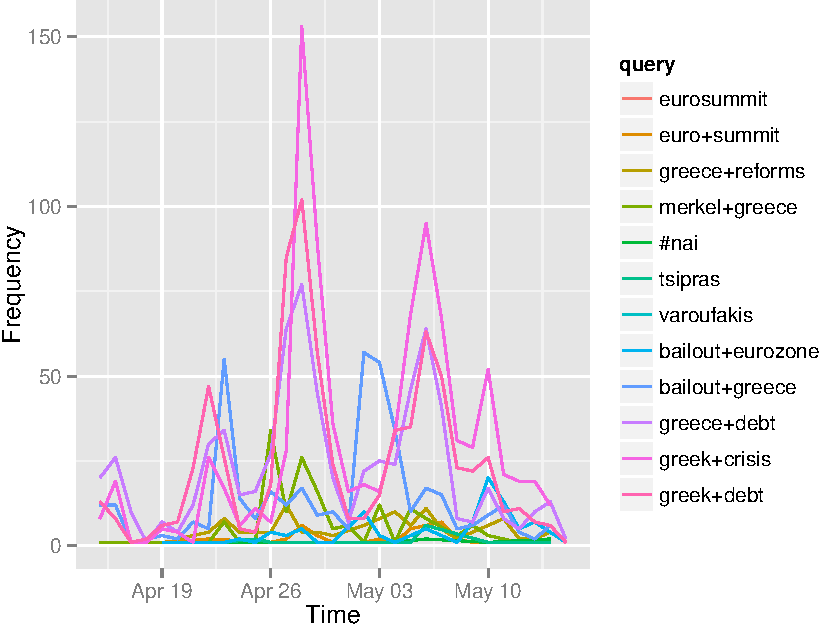
\includegraphics{fin_paper_files/figure-latex/unnamed-chunk-8-1} 

}

\caption{Most common search queries, 2010}\label{fig:unnamed-chunk-8}
\end{figure}

In the 2010 period, ``greek+crisis'' and ``bailout+greece'' are the most
frequently used query. ``Bailout'' usage in tweets peaks around April
23rd when Greek prime minister Papandreo formally requested an
international bailout for Greece. In the following day, ``greek+crisis''
is used at its highest level, with nearly 125 occurances on April 28th.
However, the use of ``greek+crisis'' in tweets dropped dramatically for
a short period of around 6 days, before it peaked again, however
somewhat less pronounced. The drop in usage of ``greek+crisis'' was
accompanied by an increase in usage of ``greek+bailout'', which peaked
around May 2nd before it subsided. On May 2nd, the agreement on the
First bailout package was reached (Goncalves 2015). During this short
phase, ``greek+bailout'' was the most prominently used word combination
(from our sample). Only after ``greeck+crisis'' became most frequently
used words.

\begin{figure}

{\centering 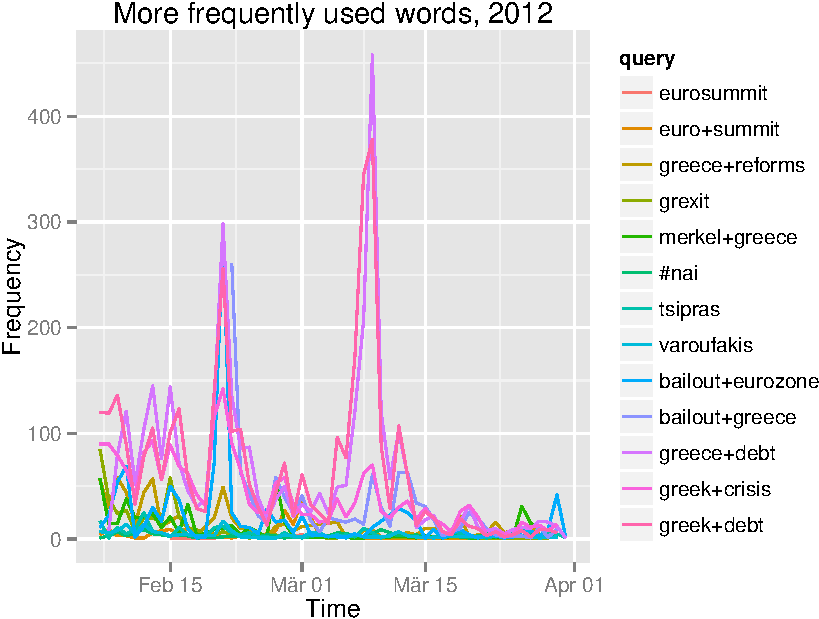
\includegraphics{fin_paper_files/figure-latex/unnamed-chunk-9-1} 

}

\caption{Most common search queries, 2012}\label{fig:unnamed-chunk-9}
\end{figure}

In the 2012 period, there was a discourse on the greek crisis weeks
before the agreement. ``greek+crisis'' was used from the beginning of
February until February 21st when the agreement between the Greek
government and the Troika was reached (Economist 2015) constantly in
between around 40 to 75 tweets. The usage of ``greek+crisis'' peaked at
the date when the agreement was reached (in contrast to 2010 when it
dropped around this phase). However, just like in 2010,
``bailout+greece'' became the most frequently used phrase in all tweets
(of our sample) at the time when agreement was reached. After that,
twitter users tweeted less about ``bailout+greece'' and
``greek+crisis''. However, it took nearly a month for those words being
used only ten times a day. Notably, ``grexit'' which had not been used
in 2010 was used frequently in the negotiation phase.

\begin{figure}

{\centering 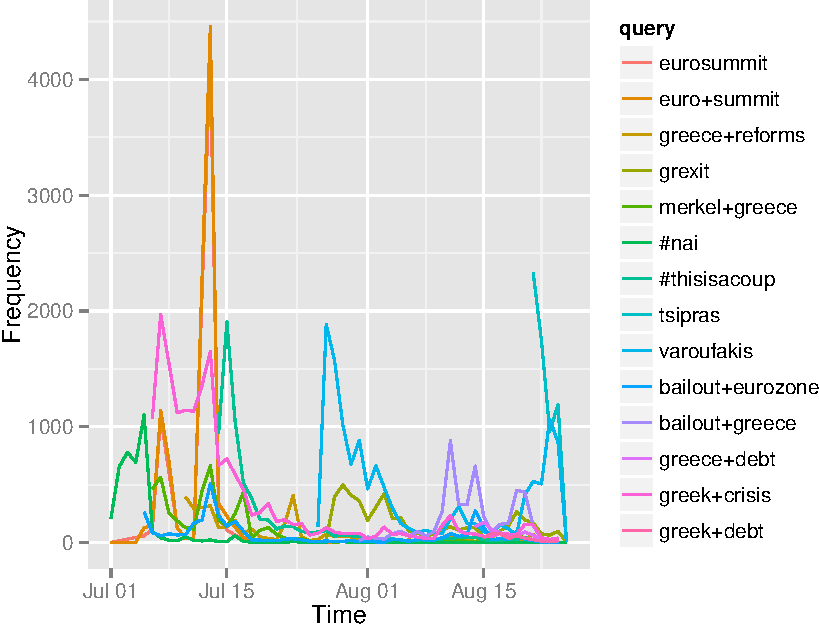
\includegraphics{fin_paper_files/figure-latex/unnamed-chunk-10-1} 

}

\caption{Most common search queries, 2015}\label{fig:unnamed-chunk-10}
\end{figure}

In the 2015 period, ``greek crisis'' was still amongst the most commonly
used words in the corpus of tweets we collected. While at its highest
peaks in 2010 and 2012 it was used around 120 times daily, we found
around 1500 occurances of ``greek+crisis'' in one day in the 2015
period. Equally popualar were ``\#ThisIsACoup'' and ``Varoufakis'', and
``Tsipras''. The most freqquently used word in the 2015 period was
``eurosummit'' which was used a lot in the time running up to the summit
and during the summit. During the summit, ``greek+crisis'' also peaked.
In the aftermath of the announcement that an agreement had been reached,
there is much less tweets. The Hashtag ``This is a Coup'' emerged on
July 14th, peaked in July 15th - equally prominent as ``greek+crisis''.
``Varoufakis'' becomes frequently used in tweets in late July, which may
have been caused by the release of an interview interview with
revelations about a previously secret ``plan B''. (Kitsantonis 2015)
``bailout+greece'' peaked around the 14th of August, when the Greek
parliament approved the third bailout package. Towards the end of the
period, ``varoufakis'' and ``tsipras'' become frequently used.
``varoufakis'' has a second peak when he resigns (on August 20th).

\newpage

\subsection{Inferential Statistics: Sentiment
Analysis}\label{inferential-statistics-sentiment-analysis}

We summarised sentiment over time and across countries. Figures 11-13
show total sentiment scores (across all queries) and sentiment variance
for all of the European countries in our dataset in each of the three
time periods. We can visually identify variation in the overall score
and in the variance between countries and across the three time periods.

\begin{figure}[htbp]
\centering
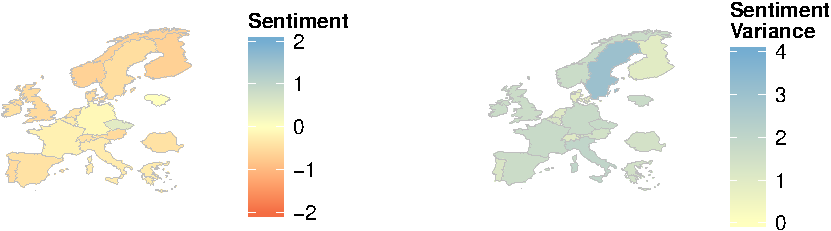
\includegraphics{fin_paper_files/figure-latex/unnamed-chunk-12-1.pdf}
\caption{Sentiment scores and variance across all search queries (2010)}
\end{figure}

\begin{figure}[htbp]
\centering
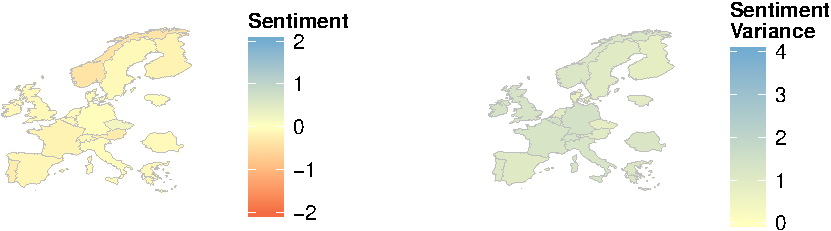
\includegraphics{fin_paper_files/figure-latex/unnamed-chunk-13-1.pdf}
\caption{Sentiment scores and variance across all search queries (2012)}
\end{figure}

\begin{figure}[htbp]
\centering
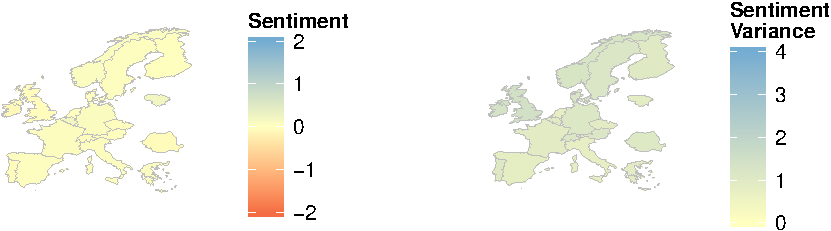
\includegraphics{fin_paper_files/figure-latex/unnamed-chunk-14-1.pdf}
\caption{Sentiment scores and variance across all search queries (2015)}
\end{figure}

To test whether the spatio-temporal distribution of sentiment in tweets
is significant, we regress sentiment score on country and time dummies.

An F-test on the joint significance of country and time finds that we
can reject at the 1\% significance level (p = 0) the null hypothesis
that time-period and country have no effect on sentiment.

We focus our analysis in this paper on the whole corpus, though we also
release our dataset aggregated at the country level in
\href{http://mcallaghan.github.io/col_res_proj/}{interactive form},
where users can investigate specific queries during any of the periods.

To focus our analysis, we zoom in to a single time period (2015), and to
two countries where we expect sentiment to diverge: Greece and Germany.
Figure 14 plots daily sentiment averages, surrounded by a band the width
of the square root of the variance. A first observation is that the
paths of the lines are remarkably similar. Following on from this, we
can see how sentiment in both countries reacts to actual political
events. On the 13th of July, Greece and its creditors struck a deal to
agree on terms for bailout funds in exchange for stringent cuts and
reforms. (Haenska and Bauchowitz 2015) identify the emergence of the
``\#thisisacoup'' hashtag on the 13th. We can observe a clear drop in
sentiment over the next two days in both countries. On the 14th of
August the Greek parliament approved the package of reforms that formed
part of the bailout deal. This time we see a spike in sentiment, once
again in both countries, but more pronounced in Germany. Indeed, where
each countries lines diverge, it is most often Greece which displays
less positive sentiment.

\begin{figure}[htbp]
\centering
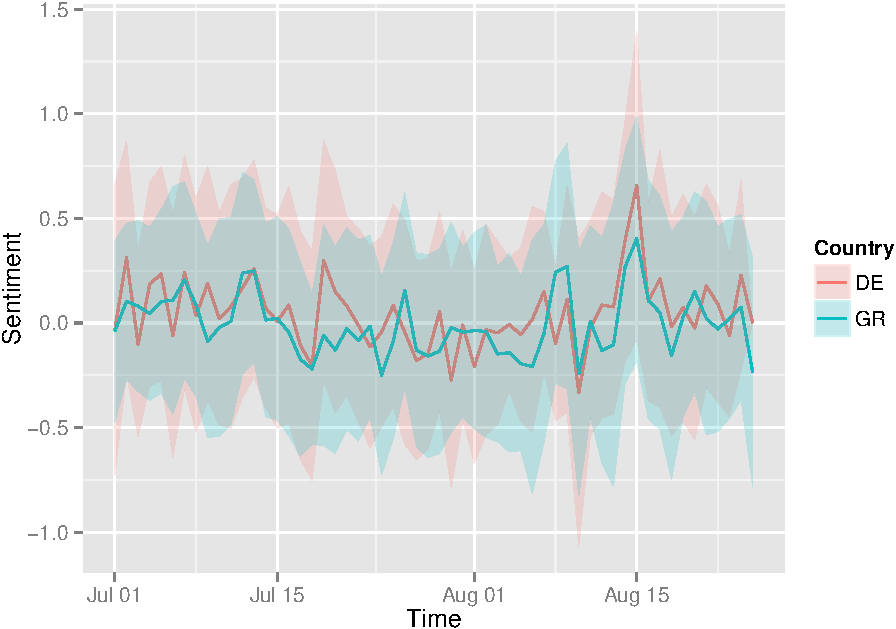
\includegraphics{fin_paper_files/figure-latex/unnamed-chunk-17-1.pdf}
\caption{Sentiment scores (line) and variance (band) for all queries in
2015}
\end{figure}

We once again regress sentiment on country and time, this time limiting
out results to 2015 period and the two countries here. In this case, the
time variable is a dummy for each day. This is intended as a control to
capture the effects of political events, but it is omitted from the
table as its interpretation is not relevant. The highly significant
negative coefficient for Greece confirms our impression from the graph
that sentiment in our corpus over this period was lower in Greece.

\begin{table}[!htbp] \centering 
  \caption{The country effect on twitter sentiment (controlling for day) in Greece and Germany in 2015} 
  \label{} 
\begin{tabular}{@{\extracolsep{5pt}}lc} 
\\[-1.8ex]\hline 
\hline \\[-1.8ex] 
 & \multicolumn{1}{c}{\textit{Dependent variable:}} \\ 
\cline{2-2} 
\\[-1.8ex] & Tweet sentiment score \\ 
\hline \\[-1.8ex] 
 Greece & $-$0.038$^{***}$ \\ 
  & (0.012) \\ 
  & \\ 
 Constant (Germany) & $-$0.010 \\ 
  & (0.064) \\ 
  & \\ 
\hline \\[-1.8ex] 
Observations & 31,893 \\ 
R$^{2}$ & 0.020 \\ 
Adjusted R$^{2}$ & 0.019 \\ 
Residual Std. Error & 0.983 (df = 31836) \\ 
F Statistic & 11.808$^{***}$ (df = 56; 31836) \\ 
\hline 
\hline \\[-1.8ex] 
\textit{Note:}  & \multicolumn{1}{r}{$^{*}$p$<$0.1; $^{**}$p$<$0.05; $^{***}$p$<$0.01} \\ 
\end{tabular} 
\end{table}

\section{Conclusion}\label{conclusion}

With respect to the first part of our research question, we receive a
clear indication that discussion over Twitter of the public debt crisis
in Greece has increased over the three time-periods we looked at. This
could be in part driven by our selection of queries, which, because the
issues and personalities associated with the most recent period are more
easily recalled, may be biased towards the most recent period. However,
the magnitude of the difference in numbers in each period suggests that
this can not be more than part of the explanation. Indeed, a quick look
at the number of tweets for what would seem to be a time-agnostic query
in figure 15, ``greek+crisis'', still suggests an exponential increase
in tweet numbers.

\begin{figure}

{\centering 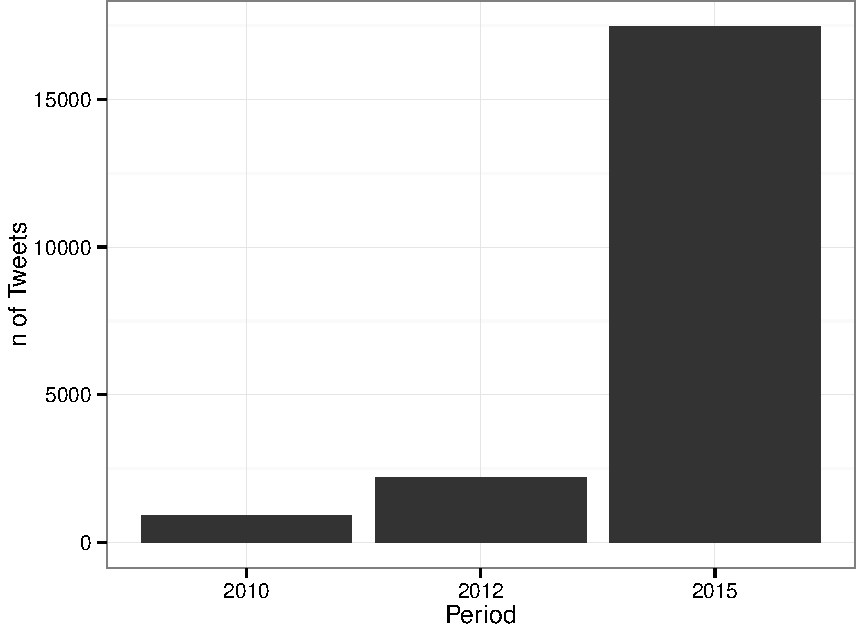
\includegraphics{fin_paper_files/figure-latex/unnamed-chunk-19-1} 

}

\caption{Tweets matching the query "greek+crisis" by year}\label{fig:unnamed-chunk-19}
\end{figure}

Assuming that discussion of the Greek crisis in the twittersphere has
increased dramatically, we cannot suggest that Europeans are talking
about European issues more. What we can say is that Europeans are
talking about European issues more on Twitter. That in itself is
significant. When Europeans communicate via the Twittersphere, all of
Europe can read that communication, and all of Europe can reply. The
same machine-translation technology that allows us to analyse a
multilingual corpus of tweets is also provided to twitter users when
browsing Twitter. Twitter therefore clearly has the potential to enable
a European public sphere. That more Europeans use are using Twitter to
talk about political issues, and that, as (Haenska and Bauchowitz 2015)
showed, tweets and replies are interconnected across countries can be
seen as positive signs for the emergence of a European public sphere.

We also showed how the content of tweets can be machine-processed at
scale (the number of tweets in our European database was 119821 and the
corpus contained 9916744 characters). The results need further
validation, and substantive interpretation is difficult, but we are able
to detect significant variation in sentiment that makes intuitive sense.
We were able, building on the work of (Haenska and Bauchowitz 2015) to
show how sentiment, as well as volume, of tweets reacted to political
events. We saw predictable differences in sentiment between countries.
The possibilities of large-scale sentiment analysis of tweets are
demonstrated. The methods developed in this paper could have significant
and varied applications.

\newpage

\section{Limitations}\label{limitations}

Some limitations to our project should be noted.

Regarding our research design, one possible limitation is our case
selection. We chose a case with a) high relevance to all European states
which also, by definition, b) divides along national lines. By comparing
Greece and Germany we did indeed find that twitter users in both
countries react to the same real world events, but we also find, that
there is a statistically significant difference in sentiment in between
the countries. To which extent these results are only characteristic for
our case or for the emergence of a common European public sphere, cannot
be answered here. Drewski in his recent contribution notes that there is
``some evidence that Europeans have reacted to the crisis not by banding
together, but by rallying around national values and interests. For
example, the German center‐left was not ready to side with the Spanish
center‐left to fight the neoliberal response to the crisis. Instead,
they preferred to stick to their German compatriots from the
center‐right in supporting austerity politics.'' He further assesses
that ``this is no good news for the idealists' vision of a European
demos engendered by the Euro crisis. A post‐national European democracy,
giving voice to transnational political coalitions, is still far from
becoming reality.'' (Drewski, Gerhards, and others 2015)

Regarding data processing, the limitations should be mentioned. Location
plays a crucial role in our research design. For most of the location
data we relied on the location provided by the user themselves. As
mentioned earlier, Devin Gaffney already pointed out methodological
problems with using the given location of twitter users - ``in many
cases user-entered profile locations differ from the physical locations
users are actually Tweeting from'' (Graham, Hale, and Gaffney,Devin
2014, 1). Additionally, we did not translate all tweets (namely, we did
not translate Danish and Romanian tweets). This was because the error
rate when identifying tweets written in those languages was very high.
Hence, the results for those countries should be read carefully, as they
mirror sentiment in those tweets written in English.

\section*{References}\label{references}
\addcontentsline{toc}{section}{References}

Annau, Mario. 2014. \emph{Tm.plugin.sentiment: Text Corpus Sentiment
Analysis}. \url{http://R-Forge.R-project.org/projects/sentiment/}.

Balahur, Alexandra, and Marco Turchi. 2012. ``Multilingual Sentiment
Analysis Using Machine Translation?'' \emph{Proceedings of the 3rd
Workshop in Computational Approaches to Subjectivity and Sentiment
Analysis P. 52-60}.
\url{http://publications.jrc.ec.europa.eu/repository/handle/JRC73293}.

Biernacki, Patrick, and Dan Waldorf. 1981. ``Snowball Sampling: Problems
and Techniques of Chain Referral Sampling.'' \emph{Sociological Methods
\& Research} 10 (2). SAGE Publications: 141--63.

Drewski, Daniel, J{ü}rgen Gerhards, and others. 2015. ``Has There Been a
European Public Discourse on the Euro Crisis?''

Economist, The. 2015. ``Greece's Return to the Markets.'' Accessed
December 3.
\url{http://www.economist.com/news/finance-and-economics/21600727-bond-issue-milestone-there-still-long-way-go-prodigal-son}.

Gentry, Jeff. 2015. \emph{TwitteR: R Based Twitter Client}.
\url{http://CRAN.R-project.org/package=twitteR}.

Goncalves, Sergio. 2015. ``Markets Calm Amid New Austerity for
Portugal.'' Accessed December 3.
\url{http://www.reuters.com/article/2010/05/14/us-eurozone-idUSTRE6400PJ20100514}.

Graham, Mark, Scott a. Hale, and Gaffney,Devin. 2014. ``Where in the
world are you ? Geolocation and language identification in Twitter.''
\emph{The Professional Geographer} 00 (2013): 00.
doi:\href{http://dx.doi.org/10.1080/00330124.2014.907699}{10.1080/00330124.2014.907699}.

Grimmer, Justin, and Brandon M Stewart. 2013. ``Text as Data: The
Promise and Pitfalls of Automatic Content Analysis Methods for Political
Texts.'' \emph{Political Analysis}. SPM-PMSAPSA, mps028.

Haenska, Max, and Stefan Bauchowitz. 2015. ``A European Twitter Sphere?
What Tweets on the Greek Bailout Say About How Europeans Interact
Online.'' Accessed October 23. \url{http://perma.cc/6ZVZ-X5GT}.

Henrique, Jefferson. 2015. ``Get Old Tweets Programmatically.'' Accessed
October 21. \url{https://github.com/Jefferson-Henrique/GetOldTweets}.

Hornik, Kurt, Johannes Rauch, Christian Buchta, and Ingo Feinerer. 2015.
\emph{Textcat: N-Gram Based Text Categorization}.
\url{http://CRAN.R-project.org/package=textcat}.

Hughes, Amanda Lee, and Leysia Palen. 2009. ``Twitter adoption and use
in mass convergence and emergency events.'' \emph{International Journal
of Emergency Management} 6 (May): 248.
doi:\href{http://dx.doi.org/10.1504/IJEM.2009.031564}{10.1504/IJEM.2009.031564}.

Jungherr, Andreas, Pascal J{ü}rgens, and Harald Schoen. 2012. ``Why the
Pirate Party Won the German Election of 2009 or the Trouble with
Predictions: A Response to Tumasjan, a., Sprenger, tO, Sander, PG, \&
Welpe, IM `Predicting Elections with Twitter: What 140 Characters Reveal
About Political Sentiment'.'' \emph{Social Science Computer Review} 30
(2). SAGE Publications: 229--34.

Kitsantonis, Jack Ewing; Niki. 2015. ``Greece Made Preparations to Exit
Euro.'' Accessed December 3.
\url{http://www.nytimes.com/2015/07/28/business/greece-debt-varoufakis-recording.html?_r=1}.

Lucas, Christopher, and Dustin Tingley. 2014. \emph{TranslateR: Bindings
for the Google and Microsoft Translation APIs}.
\url{http://CRAN.R-project.org/package=translateR}.

Metz, Cade. 2015. ``Twitter Now Lets You Search for Any Tweet Ever
Sent.'' Accessed October 21.
\url{http://www.wired.com/2014/11/twitter-now-lets-search-tweet-ever-sent}.

Narr, Sascha, Michael Hulfenhaus, and Sahin Albayrak. 2012.
``Language-Independent Twitter Sentiment Analysis.'' \emph{Knowledge
Discovery and Machine Learning (KDML), LWA}, 12--14.

Pak, Alexander, and Patrick Paroubek. 2010. ``Twitter as a Corpus for
Sentiment Analysis and Opinion Mining.'' \emph{In Proceedings of the
Seventh Conference on International Language Resources and Evaluation},
1320--26.
doi:\href{http://dx.doi.org/10.1371/journal.pone.0026624}{10.1371/journal.pone.0026624}.

Risse, Thomas. 2003. ``An Emerging European Public Sphere? Theoretical
Clarifications and Empirical Indicators.''

---------. 2014. ``No Demos? Identities and Public Spheres in the Euro
Crisis.'' \emph{JCMS: Journal of Common Market Studies} 52 (6):
1207--15.
doi:\href{http://dx.doi.org/10.1111/jcms.12189}{10.1111/jcms.12189}.

Scola, Nancy. 2015. ``Library of Congress' Twitter Archive Is a Huge
\#FAIL.'' Accessed October 23.
\url{http://www.politico.com/story/2015/07/library-of-congress-twitter-archive-119698.html}.

``The Search API.'' 2015. https://dev.twitter.com/rest/public/search.
Accessed October 21.

Theussl, Stefan, Paul Hofmarcher, and Kurt Hornik. 2015.
\emph{Tm.lexicon.GeneralInquirer: General Inquirer Categories}.

Tornes, Adam. 2015. ``Instant and Complete Access to Every Historical
Public Tweet.''
\url{https://blog.twitter.com/2015/full-archive-search-api}.

Trenz, Hans-Jörg. 2015. ``Europeanising the Public Sphere -- Meaning,
Mechanisms, Effects.'' In \emph{Interdisziplinäre Europastudien}, edited
by Ulrike Liebert and Janna Wolff, 233--51. Springer Fachmedien
Wiesbaden.
doi:\href{http://dx.doi.org/10.1007/978-3-658-03620-1_11}{10.1007/978-3-658-03620-1\_11}.

Tumasjan, Andranik, Timm Oliver Sprenger, Philipp G Sandner, and Isabell
M Welpe. 2010. ``Predicting Elections with Twitter: What 140 Characters
Reveal About Political Sentiment.'' \emph{ICWSM} 10: 178--85.

Vilares, David, Miguel A Alonso, and Carlos G{ó}mez-Rodr{i}guez. 2015.
``Sentiment Analysis on Monolingual, Multilingual and Code-Switching
Twitter Corpora.'' In \emph{6TH WORKSHOP oN COMPUTATIONAL APPROACHES tO
SUBJECTIVITY, SENTIMENT aND SOCIAL MEDIA ANALYSIS WASSA 2015}, 2.

Weller, Katrin, Axel Bruns, Jean Burgess, Merja Mahrt, and Cornelius
Puschmann. 2013. \emph{Twitter and Society}. Vol. 89. Peter Lang New
York.

Zimmer, Michael. 2010. ``Is It Ethical to Harvest Public Twitter
Accounts Without Consent?''
\url{http://www.michaelzimmer.org/2010/02/12/is-it-ethical-to-harvest-public-twitter-accounts-without-consent/}.

Zimmer, Michael, and Nicholas John Proferes. 2014. ``A topology of
Twitter research: disciplines, methods, and ethics.'' \emph{Aslib
Journal of Information Management} 66 (3): 250--61.
doi:\href{http://dx.doi.org/10.1108/AJIM-09-2013-0083}{10.1108/AJIM-09-2013-0083}.

\end{document}
